\documentclass[tikz,border=6pt]{standalone}
\usepackage{amsmath,amssymb}
\usepackage{xcolor}
\usetikzlibrary{arrows.meta,positioning,calc}

\begin{document}
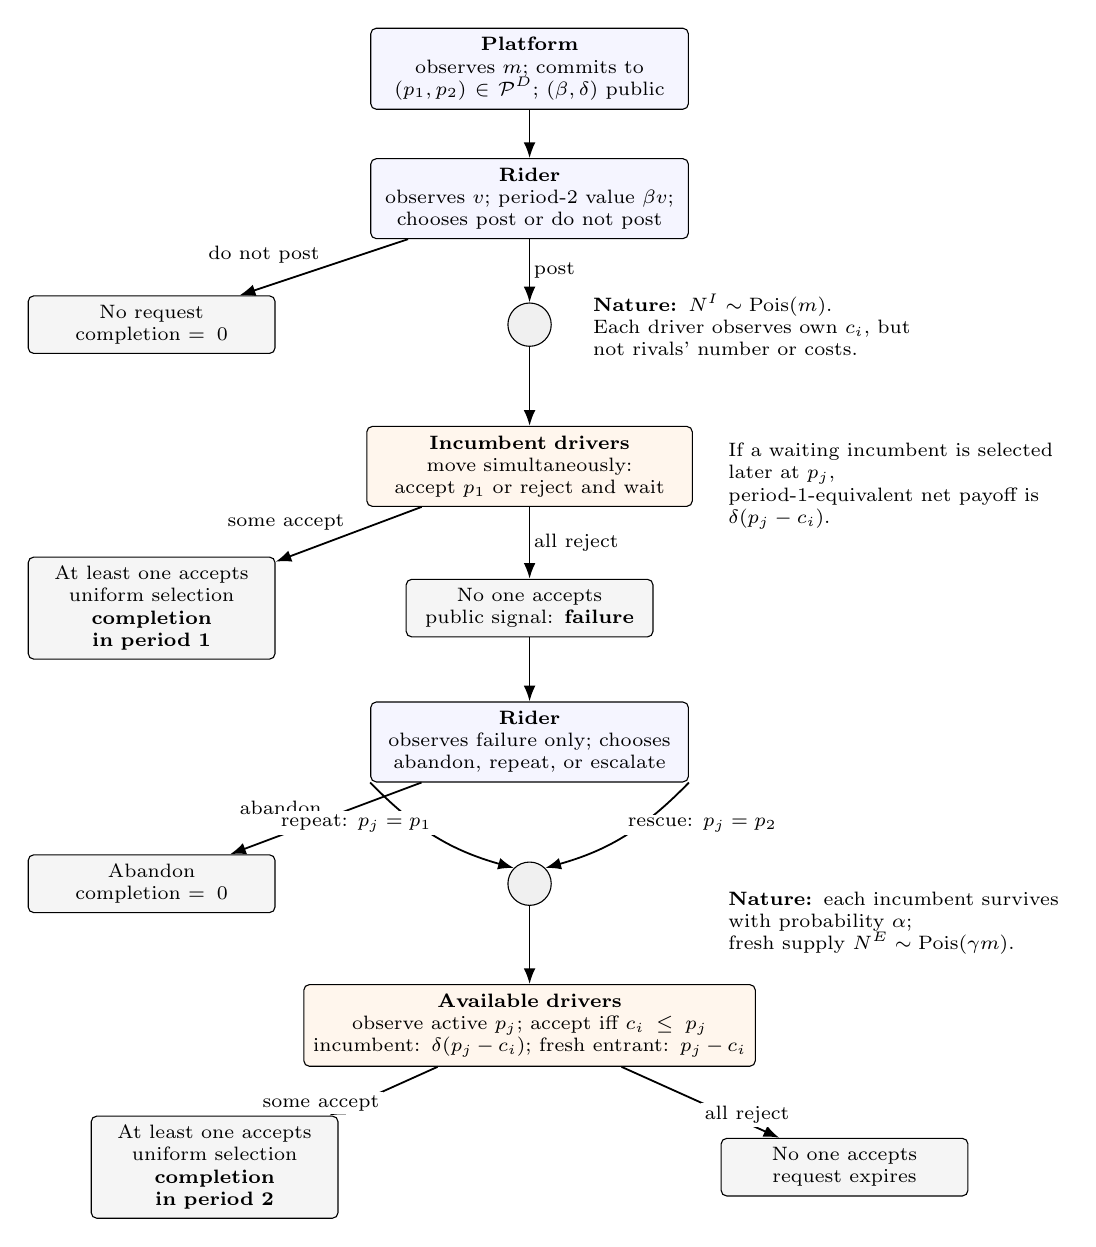
\begin{tikzpicture}[
  x=1cm,
  y=1cm,
  >={Latex[length=2mm]},
  flow/.style={->,line width=.65pt},
  decision/.style={draw,rounded corners=2pt,align=center,
    fill=blue!4,minimum height=8mm,text width=38mm,font=\scriptsize},
  driver/.style={draw,rounded corners=2pt,align=center,
    fill=orange!7,minimum height=9mm,text width=39mm,font=\scriptsize},
  terminal/.style={draw,rounded corners=2pt,align=center,
    fill=gray!8,minimum height=7mm,text width=29mm,font=\scriptsize},
  chance/.style={circle,draw,fill=gray!12,minimum size=5.5mm,inner sep=0pt},
  labeltext/.style={align=left,font=\scriptsize,text width=42mm},
  action/.style={font=\scriptsize,fill=white,inner sep=1.2pt}
]

\node[decision] (platform) at (0,0)
  {\textbf{Platform}\\observes $m$; commits to\\$(p_1,p_2)\in\mathcal P^D$; $(\beta,\delta)$ public};
\node[decision] (rider0) at (0,-1.65)
  {\textbf{Rider}\\observes $v$; period-2 value $\beta v$;\\chooses post or do not post};
\node[terminal] (nopost) at (-4.8,-3.25)
  {No request\\completion $=0$};

\node[chance] (nature1) at (0,-3.25) {};
\node[labeltext,right=4mm of nature1] (nature1text)
  {\textbf{Nature:} $N^I\sim\operatorname{Pois}(m)$.\\
   Each driver observes own $c_i$, but not rivals' number or costs.};

\node[driver] (drivers1) at (0,-5.05)
  {\textbf{Incumbent drivers}\\move simultaneously:\\accept $p_1$ or reject and wait};
\node[labeltext,anchor=west] (discountnote) at (2.4,-5.3)
  {If a waiting incumbent is selected later at $p_j$,\\
   period-1-equivalent net payoff is $\delta(p_j-c_i)$.};
\node[terminal] (complete1) at (-4.8,-6.85)
  {At least one accepts\\uniform selection\\\textbf{completion in period 1}};
\node[terminal] (failure) at (0,-6.85)
  {No one accepts\\public signal: \textbf{failure}};

\node[decision] (rider1) at (0,-8.55)
  {\textbf{Rider}\\observes failure only; chooses\\abandon, repeat, or escalate};
\node[terminal] (abandon) at (-4.8,-10.35)
  {Abandon\\completion $=0$};

\node[chance] (nature2) at (0,-10.35) {};
\node[labeltext,anchor=west] (nature2text) at (2.4,-10.85)
  {\textbf{Nature:} each incumbent survives with probability $\alpha$;\\
   fresh supply $N^E\sim\operatorname{Pois}(\gamma m)$.};
\node[driver,text width=55mm] (drivers2) at (0,-12.15)
  {\textbf{Available drivers}\\observe active $p_j$; accept iff $c_i\le p_j$\\
   incumbent: $\delta(p_j-c_i)$; fresh entrant: $p_j-c_i$};
\node[terminal] (complete2) at (-4.0,-13.95)
  {At least one accepts\\uniform selection\\\textbf{completion in period 2}};
\node[terminal] (expire) at (4.0,-13.95)
  {No one accepts\\request expires};

\draw[flow] (platform) -- (rider0);
\draw[flow] (rider0) -- node[action,above left]{do not post} (nopost);
\draw[flow] (rider0) -- node[action,right]{post} (nature1);
\draw[flow] (nature1) -- (drivers1);
\draw[flow] (drivers1) -- node[action,above left]{some accept} (complete1);
\draw[flow] (drivers1) -- node[action,right]{all reject} (failure);
\draw[flow] (failure) -- (rider1);
\draw[flow] (rider1) -- node[action,above left]{abandon} (abandon);
\draw[flow] (rider1.south west) to[bend right=15]
  node[action,above left]{repeat: $p_j=p_1$} (nature2.north west);
\draw[flow] (rider1.south east) to[bend left=15]
  node[action,above right]{rescue: $p_j=p_2$} (nature2.north east);
\draw[flow] (nature2) -- (drivers2);
\draw[flow] (drivers2) -- node[action,below left]{some accept} (complete2);
\draw[flow] (drivers2) -- node[action,below right]{all reject} (expire);

\end{tikzpicture}
\end{document}
